%导航栏===================
%指定文档类型、纸张、文字大小、板书(onecolumn or twocolumn)
\documentclass[10pt,a4paper,twocolumn]{book}
%宏包
\usepackage{ctex} %CTex宏引用 or ctexart
\usepackage{multirow} %纵向单元格合并
\usepackage{graphicx} %图片调用
\usepackage{amsmath} %AMS 数学宏集
\usepackage{amssymb}
\usepackage{fancyhdr} %页眉页脚



%标题
\title{\LaTeX}
\author{邓宁}
\date{\today}

%文段基本
\renewcommand{\baselinestretch}{1} %行距
\pagestyle{fancy}  %装饰线格式
\fancyhf{}  %格式清除

\rhead{Overleaf} 
\lhead{Guides and tutorials}
\rfoot{Page \thepage}

% \rhead{Overleaf}
% 在页眉的右侧显示大括号之中的文字。

% \lhead{Guides and tutorials}
% 在页眉的左侧显示大括号之中的文字。

% \chead{}
% 与上面的例子相似,大括号之中的文字会居中显示。

% \rfoot{Page \thepage}
% 在页脚右侧显示文字“Page”以及当前页的页码(\thepage)。文末列出了一系列自动生成内容的命令(例如章节编码等)。

% \lfoot{ }
% 在页脚左侧显示大括号之中的文字。

% \cfoot{ }
% 在页脚中间显示大括号之中的文字。

% 自定义双边文档的页面样式:
% 命令的可选参数包括:

% E:偶数页
% O:奇数页
% L:左侧
% R:右侧
% C:居中
% 例如,\fancyhead[LE,RO]{Overleaf}   (进一步的自定义)
% 会在偶数页的页眉左侧显示“Overleaf”,在奇数页的右侧显示“Overleaf”。

%自定义信息:
% \thepage
% 显示当前页的页码
% \thechapter
% 显示当前章(Chapter)的编码
% \thesection
% 显示当前节(Section)的编码
% \chaptername
% 显示文字Chapter。如果文档的默认语言不是英语,则显示Chapter的对应语言的翻译文字。
% \leftmark和\rightmark
% 显示当前文档类型的最高级文档结构的名字和编码(例如,对于报告reports和书籍books,显示Chapter;对于文章articles,显示Section)。名字大写显示。

%正文栏===================
\begin{document}  %正文开始
\maketitle  %打印标题
this is a world that is deteriorating.No one was here to live.
what is most thing letting me live? %文本输入

$f(x)$ is defined by $$f(x)=2x^2$$  %公式的初步使用

字体设置:==============================

first para
\par second para %分段(\par或者空格分段)

特殊字符:
\# \$ \% \& \{ \} \_ \^{} \~{} \textbackslash

西语连字:
\par It's difficult to find \ldots 
\par It's dif{}f{}icult to f{}ind \ldots

引号: ``Please press the `x' key.''

省略号: \dots

破折号: ---

重音与特殊字符:(详见表)

\ae \aa \AA \.a \^a \~a \r a \"a \=a\o !` ?`

上标或者公式符号可以直接引用snippet view。(tex左侧列表)

特殊字符:

\P{} \S{} \dag{} \ddag{}
\copyright{} \pounds{}
\textasteriskcentered \textperiodcentered \textbullet
\textregistered{} \texttrademark

\verb|\verb强制输出\par|

空格、换行、换栏与换页

1~2 3\\4 5 6 %手动换行\\[<pt>]
\newpage 7~~8~~~9 %在双栏排版模式中 \newpage 起到另起一栏的作用,
\clearpage 10~11 ~12  %\clearpage 则能够另起一页

章节与目录:=====================
\clearpage 章节目录附加页
\tableofcontents %生成目录
章节目录附加页
\chapter{章节}
\section[short title]{一级标题} %标题使用 ⟨title⟩ 参数,在目录和页眉页脚中使用 ⟨short title⟩ 参数;
\subsection{二级标题}
\subsubsection{三级标题} %book中没用
%\paragraph{段落}
%\part*{此命令,用来将整个文档分割为大的分块}121
\clearpage
This is the beginning of the book
\clearpage
This is the end of the book

book 文档类还提供了前言、正文、后记结构的划分命令详见lshort-zh

引用与标注:================

\subsection{交叉引用:}
% 注释快捷键 ctrl + /
%交叉引用是 L AT EX 强大的自动排版功能的体现之一。在能够被交叉引用的地方,
% 如章节、公 式、图表、定理等位置使用 \label 命令:
% \label{⟨label-name⟩} 
% 之后可以在别处使用 \ref 或 \pageref 命令,
% 分别生成交叉引用的编号和页码: \ref{⟨label-name⟩} 
%   \pageref{⟨label-name⟩} \eqref{label-name}

A reference to this subsection 
\label{sec:this} looks like: 
``see section~ \ref{sec:this} on 
page~\pageref{sec:this}.''
\subsection{脚注和边注}
方法一:

“天地玄黄,宇宙洪荒。日月盈昃,辰宿列张。”\footnote{出自《千字文》。}

方法二:(表格环境、各种盒子内)
% 有些情况下(比如在表格环境、各种盒子内)使用 \footnote 并不能正确生成脚注。
% 我们 可以分两步进行,先使用 \footnotemark 为脚注计数,再在合适的位置用 
% \footnotetext 生成 脚注。

\begin{tabular}{l l} 
    \hline
    “天地玄黄,宇宙洪荒。日月盈昃,辰宿\\列张。”
    \footnotemark \\ 
    \hline
\end{tabular} 
    \footnotetext{表格里的名句出自《千字文》。}

边注:
    \marginpar{\footnotesize 边注较窄,不要写过多文字,最好设置较小的字号。}

\subsection{列表(环境)}
 基本有序列表enumerate和无序列表itemize.
以下enumberate内的item自动编号,手动定义的item不计入编号序列
 \begin{enumerate}
    \item An item.
    \begin{enumerate}
    \item A nested item.\label{itref} 
    \item[*] A starred item.
    \item A good item
    \item[] A better item
    \end{enumerate} 
    \item Reference(\ref{itref}). 
\end{enumerate}
以下为无序编号itemize.
\begin{itemize}
    \item An item. \begin{itemize}
    \item A nested item. 
    \item[+] A `plus' item. 
    \item Another item.
    \end{itemize} 
    \item Go back to upper level. 
\end{itemize}
关键字环境 description
\begin{description}
    \item[Enumerate] Numbered list. 
    \item[Itemize] Non-numbered list. 
\end{description}
\subsection{对齐(环境)}
% \begin{center} … \end{center}
% \begin{flushleft} … \end{flushleft} 
%\begin{flushright} … \end{flushright}
除此之外,还可以用以下命令直接改变文字的对齐方式: 
% \centering \raggedright \raggedleft

例如:

\centering Centered text paragraph.\\
\raggedright Left-aligned text paragraph.\\
\raggedleft Right-aligned text paragraph.

\raggedright

\subsection{更多环境}
\begin{itemize}
    \item quote:引用环境(短)
    \item quotation:引用环境(长)
    \item abstract:摘要环境
    \item verbatim:代码环境
\end{itemize}
要排版简短的代码或关键字,可使用 \textbackslash verb 命令.
即:\\%\verb⟨delim⟩⟨code⟩⟨delim⟩
\verb|\LaTeX| \\ 
\verb+(a || b)+ \verb*+(a || b)+

\subsection{表格(环境)}
what\\
\begin{tabular}[t]{c||l r} 
    \hline \hline 
    ⟨item1⟩ & ⟨item2⟩ & ⟨item3⟩ \\
    \hline 
    ⟨item1⟩ & ⟨item2⟩ & ⟨item3⟩ \\
    \hline 
    ⟨item1⟩ & ⟨item2⟩ & ⟨item3⟩ \\
    \hline \hline 
 \end{tabular}

 列格式 \\
 
 \begin{tabular}[t]{lcr|p{6em}}%lcr是对齐方式,|为列分割,p设置单元格宽度固定为 ⟨width⟩,可自动折行
    \hline
    left & center & right
        & par box with fixed width\\
    L & C & R & P \\
    \hline
    \end{tabular}

\verb|@| 可以插入插入任意的文本,也可以适当使用以充当“竖线”。特别地,\verb|@{}| 可直接用来消除单元
格前后的间距:

\centering
\begin{tabular}[t]{@{} r@{:}lr @{|}}
    \hline 1 & 1 & one \\
     11 & 3 & eleven \\
    \hline
\end{tabular}

\raggedright
参数重复的写法 *{⟨n⟩}{⟨column-spec⟩}:

例如:

\verb+\begin{tabular}{|*{5}{c|}*{2}{p{4em}|}}+

\setlength{\parindent}{2em}
array 宏包提供了辅助格式 > 和 <,用于给列格式前后加上修饰命令

合并单元格:\\
横向合并\\
%\multicolumn{⟨n⟩}{⟨column-spec⟩}{⟨item⟩}
%n为格数、column-spec为列格式、item为内容
\begin{tabular}{|c|c|c|}
    \hline 1 & 2 & Center \\
    \hline \multicolumn{2}{|c|}{3} &
    \multicolumn{1}{r|}{Right} \\
    \hline 4 & \multicolumn{2}{c|}{C} \\
    \hline 
\end{tabular}
% 上面的例子还体现了,形如 \multicolumn{1}{⟨column-spec⟩}{⟨item⟩} 
% 的命令可以用来修 改某一个单元格的列格式。
\\
纵向合并\\
%纵向合并单元格需要用到 multirow 宏包提供的 \multirow 命令:
%\multirow{⟨n⟩}{⟨width⟩}{⟨item⟩}
%⟨width⟩ 为合并后单元格的宽度,可以填 * 以使用自然宽度。

% \usepackage{multirow} 
\begin{tabular}{ccc}
\hline 
\multirow{2}{*}{Item} &
\multicolumn{2}{c}{Value} \\ 
\cline{2-3} %定长横线
& First & Second \\ \hline 
A & 1 & 2 \\ \hline 
\end{tabular}
\\[5pt]
嵌套表格

%在以下的例子中,注意要用 \multicolumn 命令配合 @{} 格式把
%单元格的额外边距去掉,使得嵌套的表格线能和外层的表格线正确相连:

\begin{tabular}{|c|c|c|}
    \hline
    a & b & c \\ \hline a & \multicolumn{1}{@{}c@{}|}
     {\begin{tabular}{c|c}
    e & f \\ \hline e & f \\
    \end{tabular}}
    & c \\ \hline
    a & b & c \\ \hline 
\end{tabular}
\begin{tabular}{|c|c|c|}
    \hline
    a & b & c \\ \hline a & %\multicolumn{1}{@{}c@{}|}
     {\begin{tabular}{c|c}
    e & f \\ \hline e & f \\
    \end{tabular}}
    & c \\ \hline
    a & b & c \\ \hline 
\end{tabular}

\subsection{图片}
使用 latex + dvipdfmx 编译命令时,调用 graphicx 宏包时要指定
dvipdfmx 选项;而使 用 pdflatex 或 xelatex 命令编译时不需要。
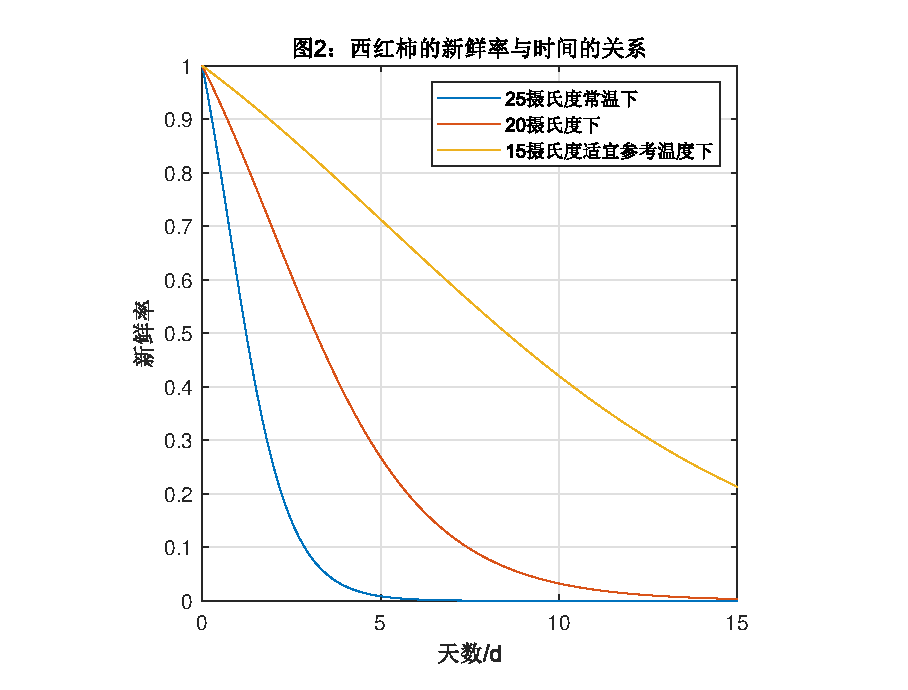
\includegraphics[width=7cm]{figures/index.eps}
%经历采用矢量图eps、figures/index.eps为相对路径

\subsection{浮动体}

环境:table or figure(* 环境用来排版跨栏的浮动体)。它们的用 法与 table 和
 figure 一样,不同之处为双栏的 ⟨placement⟩ 参数只能用 tp 两个位置
 
标序:
%\caption{…}
%  table 和 figure 两种浮动体分别有各自的生成目录的命令:
% \listoftables
% \listoffigures 
%它们类似 \tableofcontents 生成单独的章节
\begin{figure}[htbp]
    \centering
    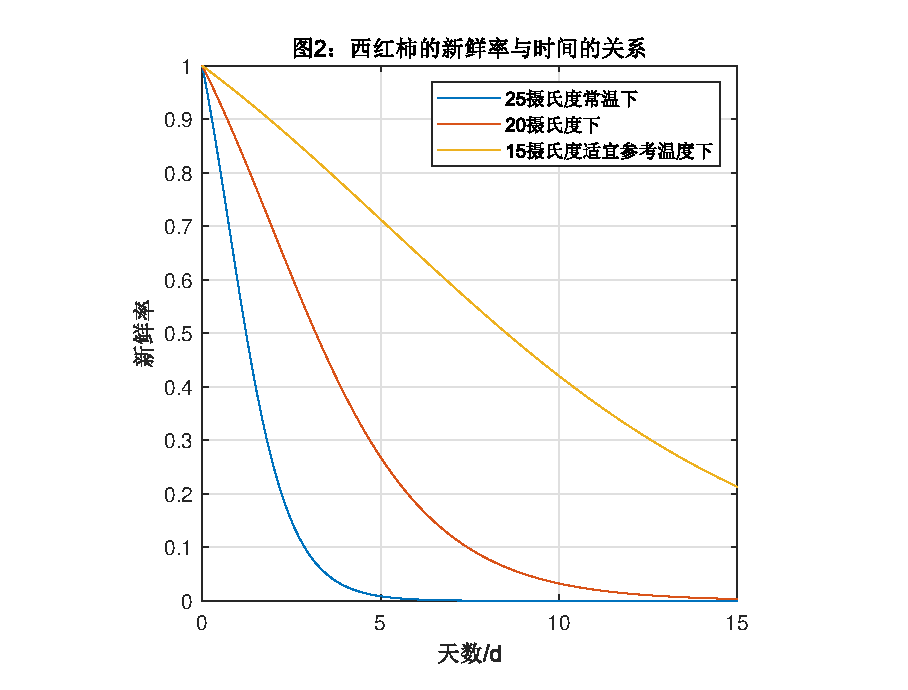
\includegraphics[width=7cm]{figures/index.eps}
    \caption{西红柿的新鲜度与时间的关系}
\end{figure}

\chapter{排版数学公式}
\section{公式排版基础}
行内公式 $a^2 + b^2 = c^2$
The Pythagorean theorem is: 
\begin{equation}
a^2 + b^2 = c^2 \label{pythagorean} 
\end{equation}
Equation \eqref{pythagorean} is called `Gougu theorem' in Chinese.

公式编号:
%\label \eqref \tag \notag 
无编号:% \[ \] or equation* or displaymath

In text: 
$\lim_{n \to \infty}
 \sum_{k=1}^n \frac{1}{k^2}
  = \frac{\pi^2}{6}$.  % 行内$局促

In display: 
\[
\lim_{n \to \infty}
 \sum_{k=1}^n \frac{1}{k^2}
  = \frac{\pi^2}{6}     % 行间\[ \] 宽敞
\]

\subsection{数学符号}
$a_1, a_2, \dots, a_n$ \\
$a_1 + a_2 + \cdots + a_n$

上下标:\\
%^ _ '
$p^3_{ij} \qquad 
m_\mathrm{Knuth}\qquad 
\sum_{k=1}^3 k $\\[5pt]
$a^x+y \neq a^{x+y}\qquad
 e^{x^2} \neq {e^x}^2$

$f(x)=x^2 \quad f'(x)=2x \quad f''^2(x)=4$

分式:

%\frac{分子}{分母} \dfrac \tfrac 令用户能够在行内使用正常大小的 分式,或是反过来
In text style: $1\frac{1}{2}$~hours \qquad $1\dfrac{1}{2}$~hours

n 次方根:

$\sqrt[n]{a}$

特殊的分式形式,如二项式结构

Pascal's rule is \[
\binom{n}{k} =\binom{n-1}{k} + \binom{n-1}{k-1}
\]

特殊关系符:\\
$\ne~\ge~\le~\approx~\equiv~\propto~\sim$

二元关系符号:\\
$~\stackrel{*}{\approx}$

算法符:\\
%× (\times)、除号 ÷ (\div)、点乘 · (\cdot)、加减号 ± (\pm) / ∓ (\mp) 
% ∇ (\nabla) 和 ∂ (\partial)
$du = \frac{\partial P}{\partial x}dx+\frac{\partial Q}{\partial y}dy
+\frac{\partial R}{\partial z}dz$\\
$\frac{d^n y}{d x^n} $
$\frac{\sin^2 x}{x}=1$

巨算符:

In text: $\sum_{i=1}^n \quad
 \int_0^{\frac{\pi}{2}} \quad
 \oint_0^{\frac{\pi}{2}} \quad 
 \prod_\epsilon $ \\
In display: \[\sum_{i=1}^n \quad 
\int_0^{\frac{\pi}{2}} \quad 
\oint_0^{\frac{\pi}{2}} \quad 
\prod_\epsilon \]
%巨算符的上下标位置可由 \limits 和 \nolimits 调整,
% 前者令巨算符类似 lim 或求和算符  ,上下标位于上下方;
% 后者令巨算符类似积分号,上下标位于右上方和右下方。
\\[5pt]
In text: $\sum\limits_{i=1}^n \quad 
\int\limits_0^{\frac{\pi}{2}} \quad 
\prod\limits_\epsilon $ \\
In display: \[\sum\nolimits_{i=1}^n \quad 
\int\limits_0^{\frac{\pi}{2}} \quad 
\prod\nolimits_\epsilon \]
%amsmath 宏包还提供了 \substack,能够在下限位置书写多行表达式
\\[5pt]
\[
\sum_{\substack{0\le i\le n \\
j\in \mathbb{R}}}
P(i,j) = Q(n) \]

具体详见snippet view\\
Accents:
$\hat{a} \dot{a} \check{a} \bar{a} \vec{a} $

\[\int_{a}^{b} f(x) \,dx \]

\section{数组和矩阵}

数列:\\
\[ \mathbf{X} = \left(
\begin{array}{cccc} 
    x_{11} & x_{12} & \ldots & x_{1n}\\
    x_{21} & x_{22} & \ldots & x_{2n}\\
    \vdots & \vdots & \ddots & \vdots\\
    x_{n1} & x_{n2} & \ldots & x_{nn}\\
\end{array} \right) \]

\[ |x| = \left\{ \begin{array}{rl}
-x & \text{if } x < 0,\\
 0 & \text{if } x = 0,\\
  x & \text{if } x > 0. 
\end{array} \right. \]

\[ |x| = \begin{cases}
 -x & \text{if } x < 0,\\
  0 & \text{if } x = 0,\\
   x & \text{if } x > 0. 
\end{cases} \]

% amsmath 宏包还直接提供了多种排版矩阵的 环境,
% 包括不带定界符的 matrix,以及带各种定界符的矩阵
% pmatrix( () )、bmatrix( [] )、Bmatrix ( {} )、
% vmatrix( ||  )、Vmatrix(  || || )。使用这些环境时,
% 无需给定列格式

\[ 
\begin{matrix} 
1 & 2 \\ 3 & 4
\end{matrix} 
\qquad \begin{bmatrix}
x_{11} & x_{12} & \ldots & x_{1n}\\
x_{21} & x_{22} & \ldots & x_{2n}\\
\vdots & \vdots & \ddots & \vdots\\
x_{n1} & x_{n2} & \ldots & x_{nn}\\
 \end{bmatrix}
\]

\[ 
\mathbf{H}= \begin{bmatrix} 
\dfrac{\partial^2 f}{\partial x^2} & 
\dfrac{\partial^2 f}
{\partial x \partial y} \\[8pt] 
\dfrac{\partial^2 f}
{\partial x \partial y} & 
\dfrac{\partial^2 f}{\partial y^2} 
\end{bmatrix}
\]

$E_n$表示第n志愿老师的平均给分,$P_n$ 表示第n志愿选中概率。
M表同级志愿和更高级志愿人数。m表示课程班最大容量.

决策模型:

\[ Max \sum_{n = 1}^{3} E_n * P_n \] 
\[s.t.~~P_n= \frac{m}{M}\]

\chapter{排版样式设定}

\section{字体设置:}
{\rmfamily rmfamily}~\textrm{rmfamily}\\
{\sffamily sffamily}~\textsf{rmfamily}\\
{\bfseries bfseries}~\textbf{bfseries}\\
{\itshape itshape}  ~\textit{itshape}\\
{\slshape slshape}  ~\textsl{slshape}

{\songti 宋体}\\
{\heiti 黑体}\\
{\kaishu 楷书}\\

\section{字号设置:}
%\fontsize{⟨size⟩}{⟨base line-skip⟩}
\fontsize{12}{14}
test1\\
test2\\[5pt]
\begin{tabular}{|*{3}{c|}}
    \hline
    {\tiny tiny}   & {\small small} &{\normalsize normalsize} \\ \hline
    {\large large} & {\Large Large} &{\LARGE LARGE}   \\ \hline
    {\huge huge}   & {\Huge Huge}   &{NULL}\\ \hline
\end{tabular}

\section{字体装饰}
\underline{underlined}\qquad \emph{emphasize}

\section{段落格式}

\subsection{段落缩进:}

{
    \setlength{\leftskip}{4em}{左缩进左缩进左缩进}\par
\setlength{\rightskip}{4em}{+右缩进右缩进右缩进} \par
\setlength{\parindent}{2em}{+首段缩进首段缩进首段缩进}\par
}
%\indent \noindent
\LaTeX 默认在段落开始时缩进,长度为用上述命令设置的 parindent。
如果需要在某一段 不缩进,可在段落开头使用 noindent 命令。相反地,
indent 命令强制开启一段首行缩进的 段落。在段落开头使用多个 indent 
命令可以累加缩进量。

\subsection{段落间距:}
设置段落间距在 0.8ex 到 1.5ex 变动:
\setlength{\parskip}{1ex plus 0.5ex minus 0.2ex}
\subsection{行距设置:}

% \renewcommand{\baselinestretch}{2} 定义了\baselinestretch的长度 (全局)


\subsection{水平间距:}
\LaTeX 默认为将单词之间的“空格”转化为水平间距
手动:
This\hspace{1.5cm}is \quad 和 \qquad a space
%\hspace* 命令代替 \hspace 命令得到不会因断行而消失的水平间距。

\subsection{垂直间距:}

{
A paragraph.

\vspace{2ex} 
Another paragraph.
}
%\vspace 命令生成的垂直间距在一页的顶端或底端可能被“吞掉”,
% 类似 \hspace 在一行的 开头和末尾那样。对应地,\vspace* 命令
% 产生不会因断页而消失的垂直间距。
\\[6pt] or \\*[6pt]

\section{页面设置}
\subsection{纸张设置}
% \usepackage{geometry}
% \geometry{a4paper,left=1.25in,right=1.25in,top=1in,bottom=1in}
\subsection{分栏}
% \onecolumn \twocolumn
\subsection{页眉页脚}
%\pagestyle{⟨page-style⟩} or \thispagestyle{⟨page-style⟩}

%empty 页眉页脚为空 
%plain 页眉为空,页脚为页码。(article 和 report 文档类默认;book 文档类
%      的每章第一页也为 plain 格式)

%headings 页眉为章节标题和页码,页脚为空。(book 文档类默认)
%myheadings 页眉为页码及 \markboth 和 \markright 命令手动指定的内容,页脚为空。

%fancyhdr 宏包 ****

正片开始:

删除当前页面页眉页脚: %\thispagestyle{empty}

自定义单边文档的页面样式:


\end{document}   %正文结束
